% DAI 2026 Industry Track Paper
% Multi-Agent Collaboration Benchmark Toolkit
% ACM format

\documentclass[sigconf,nonacm]{acmart}

% Packages
\usepackage{booktabs}
\usepackage{multirow}
\usepackage{listings}
\usepackage{xcolor}
\usepackage{graphicx}
\usepackage{subcaption}
\usepackage{hyperref}
\usepackage{tikz}
\usepackage{float}
\usetikzlibrary{arrows,shapes,positioning,fit,backgrounds}

% Tighten float spacing to reduce overlap
\setlength{\floatsep}{4pt plus 2pt minus 2pt}
\setlength{\textfloatsep}{6pt plus 2pt minus 2pt}
\setlength{\intextsep}{4pt plus 2pt minus 2pt}
\setlength{\dbltextfloatsep}{6pt plus 2pt minus 2pt}
\setlength{\dblfloatsep}{4pt plus 2pt minus 2pt}

% Metadata
\title{Multi-Agent Collaboration Benchmark: A Framework-Agnostic Toolkit for Comparing Agentic AI Systems}

\author{Junze Li}
\affiliation{%
  \institution{Nanjing University}
  \city{Nanjing}
  \country{China}
}

\begin{document}

\begin{abstract}
Multi-agent AI frameworks—CrewAI, AutoGen, LangGraph, and others—lack standardized evaluation methodologies. Most benchmarks target single-model capability rather than multi-agent collaboration quality. We present \textsc{Multi-Agent Benchmark} (MAB), an open-source, framework-agnostic toolkit providing: (1) a unified adapter interface for any agent framework; (2) a curated suite of 9 benchmark tasks across 4 categories; (3) automated instrumentation of token use, latency, cost, and overhead; and (4) an interactive visualization dashboard. Through 108 experimental runs across 12 configurations (spanning DeepSeek and OpenAI, including a real CrewAI implementation), we find that: multi-step collaboration universally improves performance (+0.05--0.16), but gains are inversely proportional to single-agent capability; simple three-stage pipelines outperform complex role-based collaboration across all tested models; and the best configuration (DeepSeek V4 Flash + multi-step) achieves 100\% success at \$0.016, 11.6$\times$ cheaper than GPT-4o.
\end{abstract}

\keywords{multi-agent systems; LLM agents; benchmark; agent evaluation; collaboration strategy; AgentOps}

\maketitle

\section{Introduction}

The landscape of AI agent development has undergone a dramatic transformation. In 2024--2026, we have witnessed the emergence of numerous multi-agent frameworks: CrewAI~\cite{crewai2024}, Microsoft's AutoGen~\cite{wu2023autogen}, LangChain's LangGraph~\cite{langgraph2024}, and many others. These frameworks enable developers to compose multiple LLM-powered agents into collaborative systems that decompose complex tasks, assign specialized roles, and—in principle—produce higher-quality outputs through structured collaboration.

However, a critical gap persists: \textbf{standardized, cross-framework evaluation is still nascent}. While recent efforts such as MAFBench~\cite{mafbench2026} have begun addressing framework comparison, they focus primarily on framework-level orchestration differences under a fixed model. Practitioners face the question—``Which framework \emph{and} which model should I use for my use case?''—with limited empirical guidance. The interaction between model choice and collaboration strategy remains underexplored. Framework selection today is often guided by documentation quality and community hype rather than measured, task-specific performance.

This problem is particularly acute for \emph{industry practitioners}. Unlike academic researchers who may evaluate on narrow RL benchmarks, industrial teams need to understand:
\begin{itemize}
    \item \textbf{Task success}: Does the multi-agent system actually solve the problem?
    \item \textbf{Cost efficiency}: How many API calls and tokens does it consume?
    \item \textbf{Time overhead}: What is the latency cost of agent coordination?
    \item \textbf{Robustness}: Does performance degrade on harder tasks or edge cases?
\end{itemize}

We introduce \textsc{Multi-Agent Benchmark} (MAB), a framework-agnostic toolkit designed to fill this gap. MAB treats each agent configuration—whether a single LLM call or a multi-step collaboration pipeline—as a unified ``black box'' behind a common adapter interface, runs identical tasks across all configurations, and produces comparative metrics. The toolkit is:
\begin{itemize}
    \item \textbf{Extensible}: New frameworks can be added by implementing a single adapter class.
    \item \textbf{Reproducible}: Tasks have deterministic inputs and automated evaluation.
    \item \textbf{Practical}: Metrics target production concerns: success rate, token cost, latency, and overhead.
    \item \textbf{Open-source}: Available under MIT license for community adoption and extension.
\end{itemize}

\section{Related Work}

\subsection{Multi-Agent Frameworks}

The past two years have seen an explosion of multi-agent frameworks. CrewAI~\cite{crewai2024} organizes agents into ``crews'' with defined roles, goals, and sequential or hierarchical task execution. AutoGen~\cite{wu2023autogen} models agent interaction as structured conversations, with group chat managers orchestrating multi-agent dialogues. LangGraph~\cite{langgraph2024} represents agent workflows as directed state graphs, providing explicit control flow. Each framework embodies different design philosophies: role-based decomposition (CrewAI), conversation-driven collaboration (AutoGen), and graph-based orchestration (LangGraph). Recent work has begun comparing these frameworks~\cite{mafbench2026,benchagent2026}, but the interaction between framework choice, model selection, and task type remains underexplored.

\subsection{LLM Evaluation Benchmarks}

Existing LLM benchmarks—MMLU~\cite{hendrycks2021mmlu}, HumanEval~\cite{chen2021humaneval}, Big-Bench~\cite{srivastava2023bigbench}, GAIA~\cite{mialon2023gaia}—evaluate single-model capabilities. They do not measure multi-agent collaboration quality. SWE-Bench~\cite{jimenez2024swebench} evaluates agents on software engineering tasks but is tied to a specific domain and does not compare frameworks. AgentBench~\cite{liu2024agentbench} evaluates single agents across diverse environments but does not address multi-agent coordination.

\subsection{AgentOps and Observability}

Recent work on AgentOps~\cite{moshkovich2025taming,dong2025taxonomy} has established the importance of observability in agentic systems. Our toolkit builds on these insights by making metric collection a first-class concern—every LLM call is instrumented, every interaction is traced, and overhead is quantified. Unlike commercial AgentOps platforms (LangSmith, AgentOps.ai, Braintrust), MAB is designed specifically for cross-framework comparison rather than production monitoring.

\subsection{Multi-Agent Evaluation}

Several recent efforts have begun addressing the framework comparison gap. MAFBench~\cite{mafbench2026} proposes an architectural taxonomy for multi-agent frameworks and provides a unified evaluation suite. BenchAgent~\cite{benchagent2026} investigates whether additional agents improve performance under normalized protocols, finding that most multi-agent systems do not exceed single-agent baselines. MASEval~\cite{maseval2026} offers a PyPI package for multi-agent system evaluation against existing benchmarks like GAIA and AgentBench.

MAB differs from these efforts in three key respects. First, we \textbf{jointly vary model tier and collaboration strategy}, revealing the model-collaboration interaction effect that prior work—which typically fixes the model—cannot observe. Second, we include \textbf{cost-performance Pareto analysis} as a first-class evaluation dimension, reflecting the practical reality that industrial adoption depends on both quality and cost. Third, our \textbf{lightweight, extensible adapter architecture} (approximately 100 lines per framework) and interactive Streamlit dashboard lower the barrier to entry for practitioners who want to benchmark their specific tasks, rather than relying on pre-packaged benchmark suites.

\section{System Design}
\label{sec:design}

\subsection{Architecture Overview}

MAB follows a modular architecture with five layers, as shown in Figure~\ref{fig:architecture}:

\begin{figure}[t]
\centering
\resizebox{\columnwidth}{!}{%
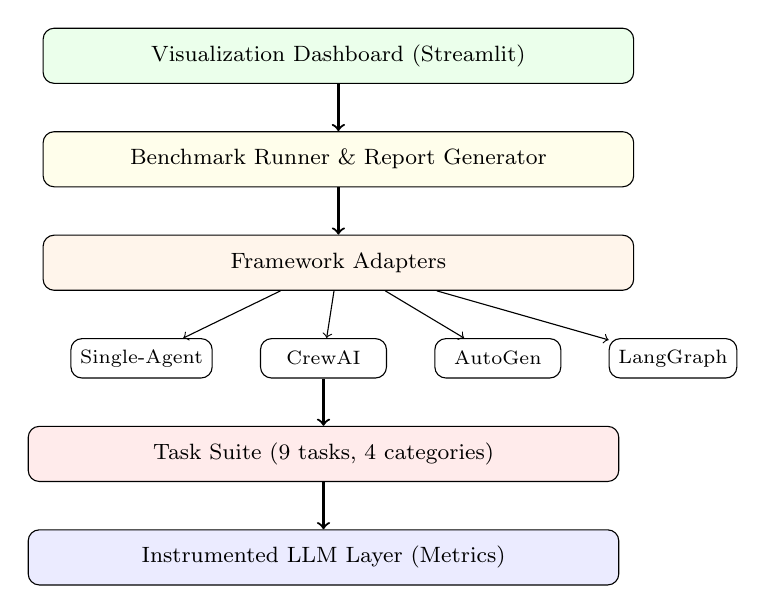
\begin{tikzpicture}[
    node distance=6mm,
    box/.style={draw, rounded corners, minimum width=7.5cm, minimum height=7mm, align=center, fill=blue!5, font=\footnotesize},
    innerbox/.style={draw, rounded corners, minimum width=1.6cm, minimum height=5mm, align=center, font=\scriptsize, fill=white},
]
\node[box, fill=green!8] (dashboard) {Visualization Dashboard (Streamlit)};
\node[box, below=of dashboard, fill=yellow!8] (runner) {Benchmark Runner \& Report Generator};
\node[box, below=of runner, fill=orange!8] (adapters) {Framework Adapters};
\node[innerbox, below=of adapters, xshift=-2.5cm] (sa) {Single-Agent};
\node[innerbox, right=of sa] (ca) {CrewAI};
\node[innerbox, right=of ca] (aa) {AutoGen};
\node[innerbox, right=of aa] (lg) {LangGraph};
\node[box, below=of ca, fill=red!8] (task) {Task Suite (9 tasks, 4 categories)};
\node[box, below=of task, fill=blue!8] (llm) {Instrumented LLM Layer (Metrics)};
%
\draw[->, thick] (dashboard) -- (runner);
\draw[->, thick] (runner) -- (adapters);
\draw[->] (adapters) -- (sa);
\draw[->] (adapters) -- (ca);
\draw[->] (adapters) -- (aa);
\draw[->] (adapters) -- (lg);
\draw[->, thick] (ca) -- (task);
\draw[->, thick] (task) -- (llm);
\end{tikzpicture}%
}
\caption{MAB architecture. The Instrumented LLM layer transparently captures all API calls. Framework adapters translate each framework's paradigm into a common interface.}
\label{fig:architecture}
\end{figure}

Our experiments (Section~\ref{sec:results}) use three adapter types—Single-Agent, Multi-Step, and Role-Based—plus a separate run with the real CrewAI library.

\subsection{Instrumented LLM Layer}

The foundation of cross-framework comparison is consistent metric collection. MAB's \texttt{InstrumentedLLM} class wraps the LLM client (supporting Anthropic, OpenAI, and DeepSeek backends) and transparently records every API call with:
\begin{itemize}
    \item Prompt and completion token counts
    \item Call duration (ms)
    \item Agent identity (which agent made the call)
    \item Call purpose (reasoning, tool invocation, summarization, etc.)
\end{itemize}

This approach ensures that metrics are collected identically regardless of which framework orchestrates the agents. All frameworks share the same underlying LLM backend with identical hyperparameters (temperature, max tokens, model version), eliminating confounding variables.

\subsection{Framework Adapters}

Each adapter implements the \texttt{BaseAdapter} interface:

\begin{lstlisting}[language=Python, basicstyle=\scriptsize\ttfamily, frame=single, breaklines=true, breakatwhitespace=false, xleftmargin=4pt, xrightmargin=4pt, columns=flexible]
class BaseAdapter(ABC):
    def solve(self, task_input: TaskInput) -> str: ...
    def run(self, task_input) -> tuple[str, RunMetrics]: ...
    def agent_names(self) -> list[str]: ...
\end{lstlisting}

The adapter is responsible for: (1) translating the benchmark task into framework-specific agent configurations, (2) executing the agents, and (3) returning the final output. This design makes adding new frameworks straightforward—approximately 100 lines of adapter code per framework.

\subsection{Task Design}

Each task in MAB is defined by three components:
\begin{itemize}
    \item \texttt{InputGenerator}: Produces deterministic task inputs with problem descriptions and structured data.
    \item \texttt{Evaluator}: Scores the output string on a 0.0--1.0 scale using keyword matching, test case execution (for code tasks), or structured answer verification.
    \item \texttt{Metadata}: Category, difficulty, recommended minimum agents, expected duration, and tags.
\end{itemize}

Tasks are designed to be \emph{inherently collaborative}—they require multiple reasoning steps, diverse knowledge, or distinct skill sets that benefit from agent specialization.

\subsection{Metrics}

For each (task, adapter) pair, MAB collects the metrics in Table~\ref{tab:metrics}.

\begin{table}[t]
\centering
\caption{Core metrics collected per benchmark run.}
\label{tab:metrics}
\small
\begin{tabular}{@{}ll@{}}
\toprule
\textbf{Metric} & \textbf{Description} \\
\midrule
Score & Task success (0.0--1.0, automated evaluation) \\
Total Tokens & Sum of prompt + completion tokens \\
Prompt Tokens & Tokens consumed by input context \\
Completion Tokens & Tokens generated as output \\
Total Time (ms) & Wall-clock duration of the run \\
Agent Interactions & Inter-agent message exchanges \\
Estimated Cost (USD) & Based on model-specific pricing \\
Orchestration Overhead & Time spent outside LLM calls \\
Efficiency Ratio & Completion tokens / total tokens \\
\bottomrule
\end{tabular}
\end{table}

\section{Benchmark Task Suite}
\label{sec:tasks}

MAB includes 9 tasks across 4 categories, summarized in Table~\ref{tab:tasks}. Each task is designed to stress-test a different aspect of multi-agent collaboration.

\begin{table}[t]
\centering
\caption{Benchmark task suite overview.}
\label{tab:tasks}
\small
\begin{tabular}{@{}llcl@{}}
\toprule
\textbf{ID} & \textbf{Task} & \textbf{Category} & \textbf{Difficulty} \\
\midrule
MHQ-1 & AlphaGo HQ language & QA & Medium \\
MHQ-2 & Moon walker birth year & QA & Medium \\
MHQ-3 & Einstein's element symbol & QA & Medium \\
CODE-1 & Palindrome function & Code Gen & Medium \\
CODE-2 & Fibonacci function & Code Gen & Medium \\
DATA-1 & Sales analysis report & Data Analysis & Medium \\
RES-1 & Transformer vs Mamba & Research & Hard \\
RES-2 & Speculative decoding & Research & Hard \\
PLAN-1 & Conference organization & Planning & Medium \\
\bottomrule
\end{tabular}
\end{table}

\subsection{Multi-hop QA (MHQ-1,2,3)}

These tasks require chaining multiple facts across reasoning steps (e.g., AlphaGo creator $\rightarrow$ HQ location $\rightarrow$ official language). Single agents may skip intermediate steps; multi-agent verification helps.

\subsection{Code Generation + Review (CODE-1,2)}

Tasks require generating correct code that passes test cases. The multi-agent workflow mimics development: one agent writes, another reviews, a third finalizes. Evaluation runs actual Python tests.

\subsection{Data Analysis (DATA-1)}

Given tabular sales data, agents must compute totals, identify trends, and produce a structured report. This requires calculation accuracy, domain reasoning, and clear communication—skills that benefit from role specialization.

\subsection{Research Synthesis (RES-1,2)}

Require deep domain knowledge and the ability to structure comprehensive explanations. Multiple agents research different aspects in parallel.

\subsection{Planning (PLAN-1)}

Tests systematic organization, constraint reasoning, and production of actionable plans with quantitative estimates.

\section{Experimental Results}
\label{sec:results}

\subsection{Experimental Setup}

We evaluate twelve configurations across four model types from two providers, including a real CrewAI~\cite{crewai2024} implementation to validate our adapter-based findings:

\begin{itemize}
    \item \textbf{DeepSeek V4 Flash} (285B/13B active, \$0.14/\$0.28 per 1M tokens) and \textbf{DeepSeek V4 Pro} (1.6T/49B active, \$0.435/\$0.87).
    \item \textbf{GPT-4o Mini} and \textbf{GPT-4o} (OpenAI, via API proxy). Cost estimates use official pricing; actual proxy costs may vary.
\end{itemize}

For each model, we test: (1) \textbf{Single-Agent} (all 4 models); (2) \textbf{Multi-Step}—a three-stage pipeline Researcher$\rightarrow$Analyst$\rightarrow$Writer (all 4 models); (3) \textbf{Role-Based}—the pipeline with CrewAI-style role definitions, backstories, and delegation (V4 Flash, GPT-4o Mini, GPT-4o); and (4) \textbf{Real CrewAI} (v1.14)—the actual library with native DeepSeek integration (V4 Flash). V4 Pro was excluded from role-based and CrewAI strategies due to its strong single-agent baseline (0.80) and higher cost. All runs use temperature$=$0.0, single repetition. Total: 108 runs (9 tasks $\times$ 12 configurations). API cost: \$0.60.

\subsection{Overall Performance}

Figure~\ref{fig:scores} and Table~\ref{tab:results} present the aggregate results. Three findings stand out:

\begin{figure}[t]
\centering
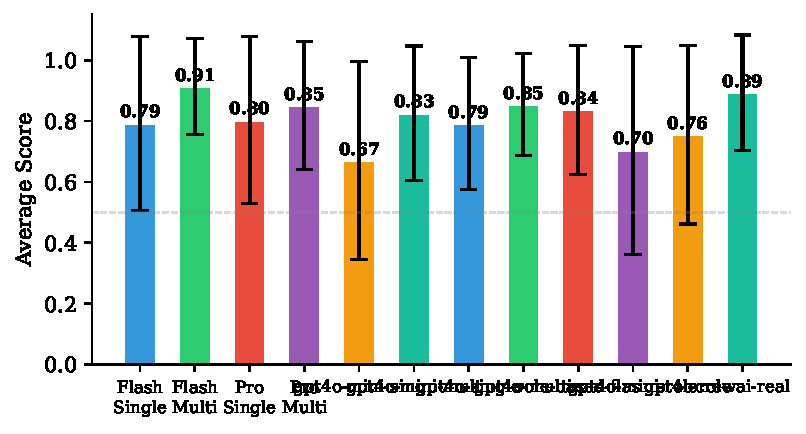
\includegraphics[width=0.88\columnwidth]{figures/score_comparison.pdf}
\caption{Average task scores across all 12 configurations. Multi-step and role-based collaboration consistently outperform single-agent baselines across all model tiers and providers.}
\label{fig:scores}
\end{figure}

\begin{enumerate}
    \item \textbf{DeepSeek V4 Flash + Multi-Step achieves the best overall result} (0.91, 100\% success rate), outperforming all other configurations including those using substantially more expensive models (V4 Pro, GPT-4o).
    \item \textbf{Multi-step collaboration universally improves performance.} Every model benefits from the Researcher-Analyst-Writer pipeline, with gains ranging from +0.05 to +0.16 in average score.
    \item \textbf{Success rate converges to 100\%} for the best multi-step configurations (V4 Flash, GPT-4o), suggesting that structured collaboration can compensate for lower single-pass capability.
\end{enumerate}

\begin{table}[t]
\centering
\caption{Aggregate results across all 9 tasks.}
\label{tab:results}
\footnotesize
\begin{tabular}{@{}lrrrrr@{}}
\toprule
\textbf{Configuration} & \textbf{Score} & \textbf{Succ.} & \textbf{Tokens} & \textbf{Time(s)} & \textbf{Cost} \\
\midrule
V4 Flash Single & 0.79 & 78\% & 13,615 & 11.6 & \$0.004 \\
V4 Flash Multi & \textbf{0.91} & \textbf{100\%} & 69,584 & 41.5 & \$0.016 \\
V4 Pro Single & 0.80 & 89\% & 13,007 & 27.1 & \$0.011 \\
V4 Pro Multi & 0.85 & 89\% & 89,386 & 164.2 & \$0.064 \\
GPT-4o Mini Single & 0.67 & 67\% & 6,256 & 8.3 & \$0.003 \\
GPT-4o Mini Multi & 0.83 & 78\% & 37,254 & 28.1 & \$0.014 \\
GPT-4o Single & 0.79 & 89\% & 5,972 & 5.5 & \$0.047 \\
GPT-4o Multi & 0.85 & 100\% & 30,496 & 19.7 & \$0.184 \\
V4 Flash Role-Based & 0.84 & 89\% & 77,799 & 60.7 & \$0.017 \\
GPT-4o Mini Role-Based & 0.70 & 67\% & 36,470 & 25.3 & \$0.012 \\
GPT-4o Role-Based & 0.76 & 78\% & 35,586 & 20.2 & \$0.203 \\
V4 Flash CrewAI & 0.89 & 89\% & N/A & 44.6 & N/A \\
\bottomrule
\end{tabular}
\par\vspace{2pt}\footnotesize CrewAI v1.14 does not expose per-task token counts through its public API; cost is excluded.
\end{table}

\subsection{The Universal Collaboration Bonus}

Figure~\ref{fig:heatmap} visualizes the collaboration effect across all task-adapter pairs. The most important finding is cross-provider universality: \textbf{the collaboration bonus holds across all four model types, but its magnitude varies inversely with single-agent capability}. GPT-4o Mini, the weakest single agent (0.67), gains the most from collaboration (+0.16). GPT-4o and V4 Pro, the strongest single agents (0.79--0.80), gain the least (+0.05--0.06). V4 Flash occupies a sweet spot—strong single-agent performance (0.79) that still benefits substantially from collaboration (+0.12).

\begin{figure}[t]
\centering
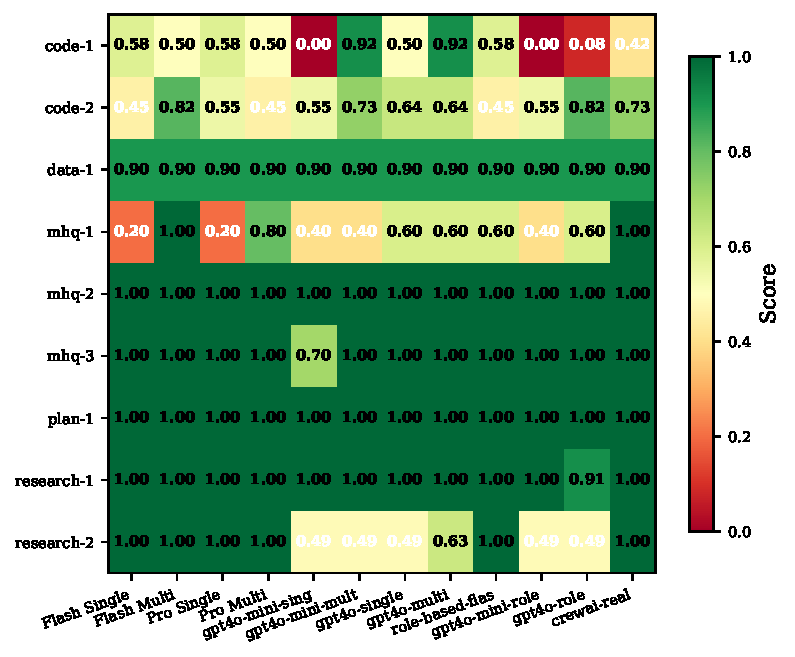
\includegraphics[width=0.88\columnwidth]{figures/heatmap.pdf}
\caption{Task $\times$ Configuration score heatmap. Collaboration configurations consistently outperform single-agent baselines (greener columns). Code tasks show the largest gains; real CrewAI approaches but does not exceed the simple multi-step pipeline.}
\label{fig:heatmap}
\end{figure}

This pattern suggests a \textbf{capability ceiling effect}: as single-agent performance approaches the task's difficulty ceiling, additional collaboration stages provide diminishing returns. The weakest models have the most headroom to benefit from structured multi-step processing.

\textbf{Role-based vs.\ simple multi-step vs.\ real CrewAI.} On V4 Flash, our simple multi-step adapter scores 0.91, real CrewAI (v1.14) scores 0.89, and our role-based adapter scores 0.84. Real CrewAI's native orchestration outperforms our role-based approximation but still falls short of the simplest three-stage pipeline—despite presumably having more engineering effort invested in its design. The role-based adapter underperforms the simpler multi-step adapter across all three tested models: V4 Flash (0.84 vs.\ 0.91), GPT-4o Mini (0.70 vs.\ 0.83), and GPT-4o (0.76 vs.\ 0.85). The gap is widest for the weakest model (GPT-4o Mini: $-0.13$), suggesting that complex role-playing prompts may confuse less capable models. These results suggest that \textbf{structural decomposition matters more than role-playing elaboration or framework sophistication}, and this principle holds across both model tiers and providers.

\subsection{Token Economics}

Figure~\ref{fig:tokens} reveals the cost of collaboration. Multi-step configurations consume 5--7$\times$ more tokens than their single-agent counterparts across all models. The token multiplier is remarkably consistent (5.1--6.9$\times$) regardless of provider or model tier—it is a structural property of the three-stage pipeline, not a model-specific behavior.

\begin{figure}[t]
\centering
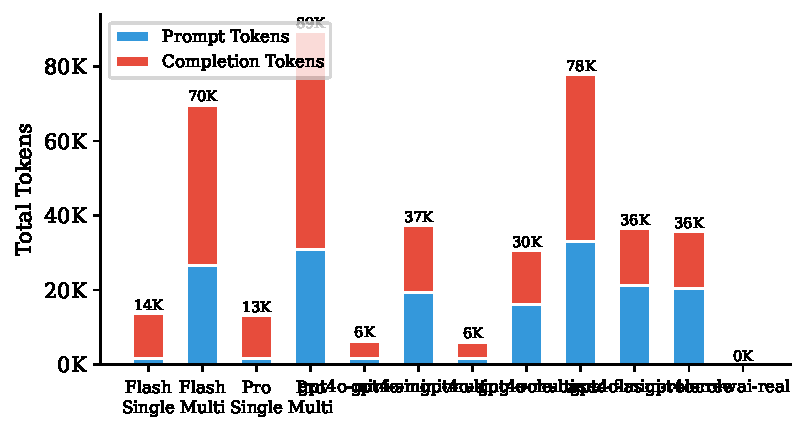
\includegraphics[width=0.88\columnwidth]{figures/token_comparison.pdf}
\caption{Token consumption across all 12 configurations. Collaboration variants consume 5--7$\times$ more tokens than single-agent baselines, dominated by prompt tokens from context handoffs.}
\label{fig:tokens}
\end{figure}

\textbf{Best value}: V4 Flash Multi achieves 100\% success at \$0.016 total—11.6$\times$ cheaper than GPT-4o Multi (\$0.184) for the same success rate. \textbf{Worst value}: V4 Pro Multi (\$0.064 for 89\% success) is Pareto-dominated by V4 Flash Multi.

\subsection{Orchestration Overhead}

Figure~\ref{fig:overhead} breaks down time into LLM computation vs.\ orchestration overhead. V4 Pro exhibits extreme overhead in multi-step mode (164s/task), driven by slower per-token generation amplified across three sequential stages. GPT-4o is the fastest single agent (5.5s) and maintains reasonable speed in multi-step mode (19.7s), suggesting that per-token latency, not pipeline depth, is the dominant factor in end-to-end latency.

\begin{figure}[t]
\centering
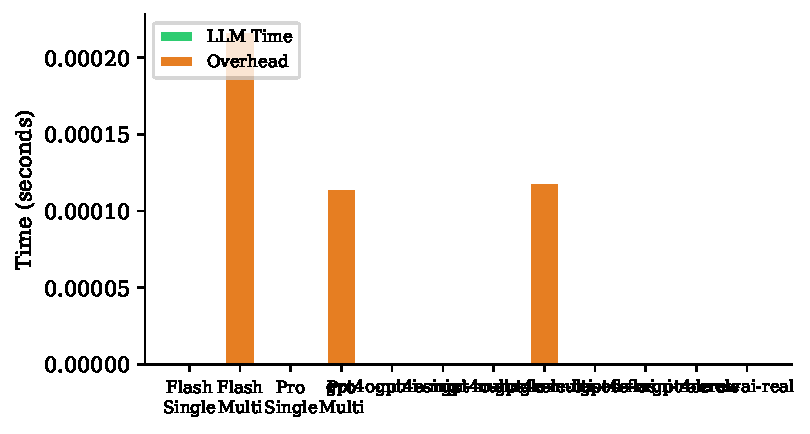
\includegraphics[width=0.88\columnwidth]{figures/overhead_comparison.pdf}
\caption{Time breakdown: LLM computation vs.\ orchestration overhead. Per-token generation speed dominates end-to-end latency; V4 Pro's slow inference makes its multi-step variant prohibitively slow.}
\label{fig:overhead}
\end{figure}

\subsection{Task-Level Findings}

\textbf{Code generation benefits most from collaboration.} CODE-1 (palindrome) shows the most dramatic improvement: GPT-4o Mini scores 0.00 as a single agent but 0.92 with multi-step—the Analyst stage catches implementation errors invisible to a single pass. CODE-2 (Fibonacci) shows model-dependent results: V4 Flash improves (+0.36) and GPT-4o Mini improves (+0.18), but GPT-4o shows no change and V4 Pro slightly regresses (-0.09), highlighting that collaboration can sometimes over-correct or dilute a working solution.

\textbf{Multi-hop QA shows model-specific patterns.} MHQ-1 (AlphaGo $\rightarrow$ UK $\rightarrow$ English) is the most discriminating task. Single agents score 0.20--0.60, while multi-step raises DeepSeek Flash to 1.00. GPT-4o models plateau at 0.40--0.60 regardless of strategy, suggesting a knowledge gap rather than a reasoning failure.

\textbf{Most knowledge tasks are near-ceiling.} MHQ-2, PLAN-1, and RES-1 are scored perfectly by nearly all configurations. MHQ-3 is perfect for 11 of 12 configurations (only GPT-4o Mini Single falls short at 0.70). In contrast, Research-2 (speculative decoding) reveals a provider-level split: DeepSeek models achieve perfect scores while GPT models plateau at 0.49--0.63 regardless of strategy, suggesting differences in pre-training knowledge coverage rather than reasoning capability.


\section{Discussion}

\subsection{Interpreting the Results}

Three patterns in our data merit deeper discussion.

\textbf{Why does the collaboration bonus vary by model tier?} The capability ceiling effect—where weaker models gain more from collaboration—has a natural explanation: multi-step pipelines help most with tasks that a single pass cannot solve. GPT-4o Mini's dramatic improvement on CODE-1 (0.00 $\rightarrow$ 0.92) occurs because its single pass fails entirely, leaving maximum headroom. Conversely, V4 Pro already scores 0.80 as a single agent, and multi-step collaboration only raises it to 0.85—well short of the best observed result (0.91). The gap between its best result and the overall best likely reflects inherent capability limits that collaboration alone cannot bridge. This suggests a practical heuristic: \textbf{benchmark your single-agent performance first; if it is below 0.70, collaboration is likely worth the cost; above 0.85, it probably is not}.

\textbf{What does the provider split on RES-2 tell us?} The fact that all DeepSeek models score 1.0 on speculative decoding while all GPT models plateau at 0.49--0.63—regardless of collaboration strategy—indicates a pre-training data coverage gap, not a reasoning deficiency. This has an important implication: \textbf{collaboration amplifies reasoning but cannot create knowledge}. When a model lacks the underlying facts, adding more agents with the same knowledge gap does not help. Practitioners should diagnose whether task failures stem from knowledge gaps or reasoning failures before investing in multi-agent architectures.

\textbf{Is the three-stage pipeline optimal?} Our experiments treat the Researcher-Analyst-Writer pipeline as a fixed design, but the optimal collaboration structure likely depends on task type. CODE-1 benefited primarily from the Analyst stage (catching bugs), while MHQ-1 benefited from the Researcher stage (decomposing the reasoning chain). The Writer stage contributed output quality improvements that our coarse scoring may not capture. Future work should explore \textbf{adaptive pipeline construction}—selecting which stages to include based on task characteristics—to avoid paying the full 5--7$\times$ token multiplier when only one stage adds value.

\subsection{Limitations}

Several limitations should be noted:
\begin{itemize}
    \item \textbf{Task ceiling effects}: Only three of nine tasks (MHQ-2, PLAN-1, RES-1) were solved perfectly by nearly all configurations, but several others (MHQ-3, DATA-1) show near-ceiling scores with minimal configuration differentiation. Future versions need harder tasks to better discriminate at higher capability levels.
    \item \textbf{Scope of the ``cheaper + collaboration > expensive'' finding}: Our headline result—that a cost-efficient model with multi-step collaboration outperforms more expensive configurations—was observed on medium-difficulty tasks with mid-tier models (DeepSeek V4 Flash/Pro, GPT-4o Mini/GPT-4o). On genuinely hard software engineering tasks (e.g., SWE-bench-level debugging, multi-file refactoring, complex algorithmic reasoning), stronger single models may outperform even well-orchestrated weaker models. Our finding should be interpreted as a call to benchmark the model-strategy combination on \emph{your specific tasks} rather than as a universal prescription to always prefer cheaper models.
    \item \textbf{Task diversity}: Our 9 tasks, while spanning 4 categories, do not cover all important multi-agent use cases (e.g., negotiation, debate, tool-use chains, long-horizon planning with state tracking).
    \item \textbf{Evaluation granularity}: Automated scoring via keyword matching and test cases is coarse. Two outputs with the same score may differ substantially in quality. Human evaluation would provide finer discrimination, especially for open-ended tasks.
    \item \textbf{Collaboration pattern vs.\ framework}: Our adapters capture essential collaboration patterns (simple pipeline, role-based) but do not reflect framework-specific optimizations (parallel execution, caching, dynamic routing) that production systems like CrewAI or LangGraph may employ. However, the consistent finding that simple multi-step outperforms both our role-based adapter and real CrewAI (v1.14) on V4 Flash, and outperforms role-based across GPT-4o Mini and GPT-4o, suggests this is a property of the collaboration strategy, not an artifact of our implementation.
    \item \textbf{Single-run evaluation}: Each configuration was run once per task. Without multiple repetitions, we cannot quantify score variance due to LLM non-determinism (even at temperature=0). Reported differences of <0.05 in average score should be interpreted cautiously.
    \item \textbf{V4 Pro pricing}: We used promotional pricing for V4 Pro (\$0.435/\$0.87). At standard pricing (\$1.74/\$3.48), the cost advantage of V4 Flash would be even more pronounced.
\end{itemize}

\subsection{Future Work}

We plan to extend MAB in several directions:
\begin{enumerate}
    \item \textbf{More tasks}: Adding negotiation, debate, tool-use coordination, and long-horizon planning tasks.
    \item \textbf{More frameworks}: Integrating newer frameworks (Agno, ChatDev, MetaGPT) as they mature.
    \item \textbf{Human evaluation}: Supplementing automated scoring with human judgment, particularly for open-ended tasks.
    \item \textbf{Multi-model comparison}: Evaluating how framework performance varies with different underlying LLMs.
    \item \textbf{Failure analysis}: Categorizing and quantifying failure modes (hallucinated consensus, infinite loops, task abandonment).
\end{enumerate}

\subsection{Recommendations for Practitioners}

Based on our findings, we offer the following concrete guidance:
\begin{itemize}
    \item \textbf{Default to cost-efficient models with multi-step.} V4 Flash Multi (0.91, 100\%, \$0.016) dominates all other configurations on the cost-quality Pareto frontier.
    \item \textbf{Do not assume larger models make better agents.} GPT-4o and V4 Pro are more expensive per token, yet underperform V4 Flash with multi-step. Collaboration strategy is the deciding factor.
    \item \textbf{Profile your specific tasks.} Three of nine tasks were trivially solved by all configurations, and several others showed near-ceiling performance. If your use case is similarly saturated, multi-agent overhead may be wasted.
    \item \textbf{Start simple, escalate only where needed.} Run a single-agent baseline first. Add collaboration only for tasks where the baseline fails—code generation and multi-hop reasoning are the strongest candidates.
    \item \textbf{Watch for latency traps.} V4 Pro Multi (164s/task) and GPT-4o Multi (\$0.184) are dominated alternatives. Cost and latency can vary by 10$\times$ across configurations for the same success rate.
\end{itemize}

\section{Conclusion}

We have presented the Multi-Agent Collaboration Benchmark (MAB), an open-source toolkit for comparing multi-agent AI systems on standardized collaboration tasks. MAB addresses a critical gap in the agent engineering ecosystem: the need for lightweight, framework-agnostic evaluation that jointly considers model selection and collaboration strategy—a dimension underexplored by existing benchmarking efforts. Through a modular adapter architecture, instrumented metric collection, and a curated 9-task suite spanning 4 categories, MAB enables practitioners to make data-driven decisions about architecture selection.

Our experiments comparing twelve configurations—including a real CrewAI implementation—across four model types and two providers yield actionable insights for practitioners. The \textbf{universal collaboration bonus} means that adding a Researcher-Analyst-Writer pipeline improves every tested model. The \textbf{capability ceiling effect} means the bonus is largest where it matters most—weak models on hard tasks. The \textbf{simplicity principle}—simple pipelines outperform complex role-playing—means teams should invest in task decomposition, not prompt engineering. And the \textbf{knowledge boundary}—collaboration cannot fill factual gaps—means diagnosing failure modes before scaling agents is essential. Together, these findings suggest that the path to effective multi-agent systems lies not in larger models or more elaborate agent personas, but in matching the right collaboration structure to the right task at the right cost.

MAB is available as open-source software under the MIT license. We invite the community to contribute new tasks, adapters for additional frameworks, and harder benchmark instances that address the ceiling effects observed in this study.

\section*{Acknowledgments}

We thank the open-source communities behind CrewAI, LangChain, and DeepSeek for their tools and APIs, which made this work possible.

\bibliographystyle{ACM-Reference-Format}
\begin{thebibliography}{99}

\bibitem{crewai2024}
CrewAI. \emph{CrewAI: Framework for orchestrating role-playing AI agents}. 2024.
\url{https://github.com/crewAIInc/crewAI}

\bibitem{wu2023autogen}
Q. Wu, G. Bansal, J. Zhang, et al. \emph{AutoGen: Enabling Next-Gen LLM Applications via Multi-Agent Conversation}. Microsoft Research, 2023.

\bibitem{langgraph2024}
LangChain. \emph{LangGraph: Build language agents as graphs}. 2024.
\url{https://github.com/langchain-ai/langgraph}

\bibitem{hendrycks2021mmlu}
D. Hendrycks, C. Burns, S. Basart, et al. \emph{Measuring Massive Multitask Language Understanding}. ICLR 2021.

\bibitem{chen2021humaneval}
M. Chen, J. Tworek, H. Jun, et al. \emph{Evaluating Large Language Models Trained on Code}. arXiv:2107.03374, 2021.

\bibitem{srivastava2023bigbench}
A. Srivastava, et al. \emph{Beyond the Imitation Game: Quantifying and extrapolating the capabilities of language models}. TMLR 2023.

\bibitem{mialon2023gaia}
G. Mialon, C. Fourrier, T. Wolf, et al. \emph{GAIA: A Benchmark for General AI Assistants}. ICLR 2024.

\bibitem{jimenez2024swebench}
C.E. Jimenez, J. Yang, A. Wettig, et al. \emph{SWE-bench: Can Language Models Resolve Real-World GitHub Issues?} ICLR 2024.

\bibitem{liu2024agentbench}
X. Liu, H. Yu, H. Zhang, et al. \emph{AgentBench: Evaluating LLMs as Agents}. ICLR 2024.

\bibitem{moshkovich2025taming}
D. Moshkovich, S. Zeltyn. \emph{Taming Uncertainty via Automation: Observing, Analyzing, and Optimizing Agentic AI Systems}. IEEE/ACM ASE 2025.

\bibitem{dong2025taxonomy}
L. Dong, Q. Lu, L. Zhu. \emph{A Taxonomy of AgentOps for Enabling Observability of Foundation Model based Agents}. arXiv:2411.05285, 2025.

\bibitem{jing2024comprehensive}
Z. Jing, X. Chang, M. Zhu, et al. \emph{A Comprehensive Evaluation Framework for Multi-Agent Reinforcement Learning}. DAI 2024.

\bibitem{chan2024chateval}
C.M. Chan, W. Chen, Y. Su, et al. \emph{ChatEval: Towards Better LLM-based Evaluators through Multi-Agent Debate}. ICLR 2024.

\bibitem{mafbench2026}
A. Orogat, A. Rostam, E. Mansour. \emph{Understanding Multi-Agent LLM Frameworks: A Unified Benchmark and Experimental Analysis}. arXiv:2602.03128, 2026.

\bibitem{benchagent2026}
Y. Fu, R. Fang, J. Shao, H. Zheng, Z. Zhu, B. Luo, T. Lin. \emph{Do More Agents Help? Controlled and Protocol-Aligned Evaluation of LLM Agent Workflows}. arXiv:2606.05670, 2026.

\bibitem{maseval2026}
C. Emde, A. Rubinstein, A. Goel, A. Heakl, S. Yun, S. J. Oh, M. Gubri. \emph{MASEval: Extending Multi-Agent Evaluation from Models to Systems}. arXiv:2603.08835, 2026.

\end{thebibliography}

\end{document}
